%%%%%%%%%%%%%%%%%%%%%%%%%%%%%%%%%%%%%%%%%%%%%%%%%%%%%%%%%%%%%%%%%%%%%%%%
% Plantilla TFG/TFM
% Escuela Politécnica Superior de la Universidad de Alicante
% Realizado por: Jose Manuel Requena Plens
% Contacto: info@jmrplens.com / Telegram:@jmrplens
%%%%%%%%%%%%%%%%%%%%%%%%%%%%%%%%%%%%%%%%%%%%%%%%%%%%%%%%%%%%%%%%%%%%%%%%

\chapter{Marco Teórico}
\label{marcoteorico}


Hay muchas definiciones de inteligencia artificial (IA) pero, desde mi punto de vista, hay dos que destacan: la de Marvin Minsky y John L. Gordon. Marvin Minsky dice que la inteligencia artificial es la ciencia que hace que las máquinas o los sistemas hagan cosas que requerirían inteligencia si las hicieran los hombres. Por otra parte, John L. Gordon dice que el objetivo de la Inteligencia Artificial es crear máquinas inteligentes y, a través de esto, comprender los principios de la inteligencia. Según estas definiciones podemos decir que los sistemas de IA se caracterizan por pensar y actuar como personas de forma razonable.


Hace tiempo que la inteligencia artificial abandonó el espectro de la ciencia ficción para colarse en nuestras vidas y, aunque todavía en una fase muy inicial, está llamada a protagonizar una revolución que, como mínimo, es comparable a la que generó Internet. Sus aplicaciones en múltiples sectores —como salud, finanzas, transporte o educación, entre otros— han provocado una explosión de trabajos de investigación desde diferentes puntos de vista. Además, estas tecnologías inteligentes, están penetrando en diferentes partes de la vida humana y, a modo de ejemplo, tenemos los sistemas de transporte inteligente, que utilizan tecnologías de información y comunicación implementadas en los propios vehículos para, entre otras cosas, reducir el impacto medioambiental o aumentar la seguridad vial.


La teoría de la IA se está desarrollando desde hace una década pero, su uso, ha tenido que esperar a que se produjeran avances en el área de las tecnologías de la información ya que requiere el desarrollo de componentes informáticos, principalmente procesadores rápidos, dispositivos de memoria de alta capacidad o redes inalámbricas. Gracias a este progreso técnico, la Inteligencia Artificial contiene técnicas y medios suficientes para ser utilizada en diferentes áreas. Así, las redes neuronales, la planificación de IA, los algoritmos evolutivos, los sistemas expertos y de conocimiento, la lógica difusa, los sistemas multiagente, la regresión vectorial, la minería de datos o las técnicas de optimización, permiten su utilización en los más diversos campos. Además, hoy en día las Tecnologías de la Información (\textit{TIC}) obligan a manejar cada vez más información en muy poco tiempo, con lo que resulta inevitable construir y utilizar técnicas capaces de clasificar, e incluso predecir, la información. Estos problemas complicados se resuelven parcialmente mediante redes neuronales que utilizan el conocimiento sobre la
organización y administración de datos en el cerebro humano.


Centrándonos más en el objeto de estudio de este trabajo, los accidentes de tráfico, podemos decir que a lo largo de los últimos años diferentes estudios se han focalizado en'analizar las causas y la severidad de los mismos. En las últimas décadas, han coexistido dos vertientes relacionadas con el análisis de la severidad de los accidentes: la perspectiva de modelos estadísticos y la del aprendizaje automático (beneficiada por el aumento de los recursos computacionales). Los modelos estadísticos tienen la característica de realizar ciertas premisas sobre los datos, asumiendo que éstos se encuentran de acuerdo a una distribución de probabilidad determinada. Sin embargo, si esta premisa sobre los datos de entrada no se cumple, se pueden producir resultados erróneos. Estos métodos se han aplicado en campos relacionados con los factores que influyen en los accidentes; como el análisis de características principales en atropellos de peatones en pasos de cebra \cite{FactoresQueInfluyen2003}, o la aplicación de regresiones logísticas multinomiales que ponderan los factores que afectan a la gravedad de accidentes en motocicletas \cite{MotorcycleCrashesMultinominalStatistic}. Otros estudios se centran en comparar distintas técnicas de modelos estadísticos entre sí para este mismo problema, como comparaciones entre \glsentryfull{svm} y probit ordenado (OP) \cite{MetodosEstadisticosComparacionSVMOP}.


Por otra parte, los modelos de aprendizaje automático no realizan ninguna presuposición sobre los datos, por lo que logran un rendimiento similar o superior a los estadísticos. En la literatura existen múltiples modelos aplicados al problema de evaluación de accidentes de tráfico, como la implementación de reglas de decisión basadas en árboles de decisión evaluando la importancia de las características \cite{ArbolDecisionSeveridadDeAccidentes}, o el uso de regresiones logísticas para clasificar su severidad \cite{LogisticRegressionPrediccionAccidentes}.

Otras metodologías han sido propuestas para este problema recientemente aplicando algoritmos genéticos. Una de las propuestas más influyentes en este campo involucra el conocimiento de los usuarios de las vías de comunicación, como ingenieros de caminos o agentes de la autoridad, para el entrenamiento modelos basados en reglas de decisión utilizando un algoritmo genético multiobjetivo \glsentryfull{nsgaii}, con el objetivo de clasificar los accidentes de tráfico \cite{NSGAIIAccidentPrediction}. Además, se han realizado trabajos para entrenar, mediante programación genética, clasificadores difusos para el descubrimiento de características influyentes y relaciones importantes entre ellas \cite{GeneticProgrammingAccidents}. Es común encontrar combinaciones de diversas metodologías buscando explotar las ventajas de cada una, realizando discusiones entre estas, como puede ser la comparación de rendimiento entre algoritmos genéticos combinados con búsqueda de patrones (\glsentryshort{ps}) respecto a perceptrones multicapa (\glsentryshort{mlp}) y redes neuronales artificiales (\glsentryshort{ann}) aplicadas a la predicción de accidentes de tráfico \cite{GAPSMLPANNAccidents}, también es frecuente el uso de estos algoritmos evolutivos para optimizar los hiperparámetros de entrada de otros modelos aplicados a este problema, como la optimización de hiperparámetros de \glsentryshort{svc} mediante el algoritmo \glsentryfull{pso} para inferir la fatalidad de los accidentes \cite{SVMPSOAccidents}.


Recientemente, las técnicas de \textit{deep learning} se están mostrando muy efectivas en resolver problemas de clasificación. En consecuencia que se han aplicado a contextos relacionados con los incidentes de tráfico, como por ejemplo, la predicción de accidentes en autopistas basados en redes neuronales \cite{RedNeuronalAutopistaAccidentes}. Sin embargo, entre la gran cantidad de modelos de \textit{deep learning}, la aplicación de redes neuronales convolucionales (\glsentryshort{cnn}) ofrece resultados muy prometedores respecto a una gran cantidad de problemas, como segmentación de matrices \cite{ImageSegmentationCNNEA}, su clasificación \cite{ImageClassificationCNNEA} y reconocimiento del lenguaje \cite{LanguageRecognitionCNNEA} entre otras, incluyendo la clasificación de gravedad de accidentes \cite{OtraPrediccionConCNNs}. La naturaleza de las redes convolucionales requiere de una entrada de datos en forma de matriz. Esto implica que haya sido necesario estudiar distintas técnicas para la transformación de datos categóricos a este formato. Una de estas propuestas es el proyecto \textit{DeepInsight} \cite{DeepInsight}, que originalmente se propuso para capturar las pequeñas variaciones existentes entre secuencias de ADN. Este modelo, es capaz de aplicar transformaciones sobre datos para posicionar las características en un eje cartesiano en función de las similitudes que presenten. Otro de los métodos propuestos, relativos a las conversiones de datos a matrices, es el algoritmo \textit{F2VI}, que construye las matrices de entrada a las \glsentryshort{cnn} en función del peso asociado a cada característica del conjunto de datos \cite{TASPCNN}. Las arquitecturas \glsentryshort{cnn} son capaces de encontrar patrones en los datos de entrada \cite{CNNReviews}, y el funcionamiento básico se puede apreciar en la figura \eqref{CNNExample}. Dentro de las redes convolucionales nos encontramos frente a dos variantes: las \glsentryfull{cnn1d} y las \glsentryfull{cnn2d}. Las \glsentryshort{cnn1d} suelen proveer gran rendimiento en numerosos campos utilizando convoluciones de una dimensión sobre la matriz de entrada, muchas han sido las aplicaciones de este modelo a problemas cotidianos, como detección de fallos de motor en vehículos \cite{MotorFailureCNN1D}, clasificación de datos personales biomédicos \cite{CNN1DMedicalSignalEA}, detección de anomalías en sistemas eléctricos \cite{ElectricSystemFailureCNN1D}, etc., siendo especialmente efectivas en procesamiento de señales \cite{Conv1D_Survey}. Otro tipo de red neuronal convolucional es la de dos dimensiones, \glsentryshort{cnn2d}, que aplicando filtros de dos dimensiones sobre la entrada son capaces de aprender patrones más complejos respecto a las de una dimensión. Esto provoca que el coste computacional del uso de esta técnica sea más elevado respecto a las \glsentryshort{cnn1d}, sin embargo, estas han sido ampliamente utilizadas en tareas de muy distinta naturaleza, demostrando un gran rendimiento, como la identificación de personas mediante reconocimiento facial \cite{FaceRecognitionCNN2EA}, clasificación de documentos escaneados \cite{DocumentAnalysisCNN2DEA} o incluso para la detección de fenómenos climatológicos extremos \cite{WeatherClimateCNN2DEA}.

Como se ha comentado, estos enfoques se muestran más efectivos que los métodos estadísticos o los basados en técnicas de \textit{machine learning} más tradicionales. No obstante, existen otros muchos enfoques de aprendizaje profundo recientes en la detección de accidentes, como el basado en aplicar redes \glsentryfull{lstm} sobre \textit{tweets} capturados tiempo real \cite{DeteccionDeAccidentesPorTweets} con el objetivo de localizar la ubicación de los accidentes, o el uso de \glsentryfull{rnn} para la predicción de lesividad de los mismos \cite{RNNAccidentSeverityPrediction}.


\begin{figure}[h]
    \centering
    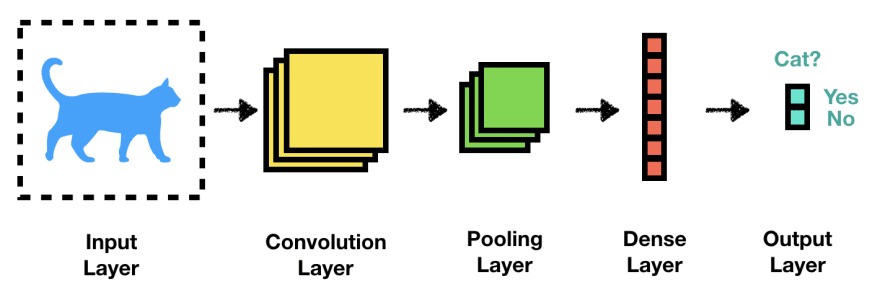
\includegraphics[width=15cm]{archivos/2.EstadoArte/CNNExample}
    \caption{Ejemplo de una red neuronal convolucional para una tarea de clasificación \cite{CNNExampleEAImage}.}
    \label{CNNExample}
\end{figure}


Uno de los principales inconvenientes comunes en estos estudios suele ser la baja calidad de los conjuntos de datos ofrecidos por las instituciones y el difícil acceso a los mismos \cite{ImportanciaDeBajaCalidadActualmenteDeDatasets}. Además, el desbalanceo de datos, asociado a la naturaleza del problema, genera una dificultad añadida a dichos estudios, ya que, en el caso de los accidentes de tráfico, gran parte de ellos suelen ser leves, siendo el número de accidentes serios y fatales mucho menor. Existen numerosos artículos que analizan este problema y se proponen distintas soluciones, como la utilización de técnicas de remuestreo \cite{ItalianoMetricasDesbalanceo} o la definición de nuevas métricas de clasificación.


Paralelamente a la predicción de gravedad de los accidentes de tráfico, existen múltiples variantes al problema que permitirían reducir el número de fallecidos en las carreteras aplicando distintas técnicas de \textit{deep learning}. Recientes investigaciones proponen arquitecturas complejas para crear mapas de riesgos de accidentes, tomando como entrada imágenes tomadas por satélite, segmentación de carreteras, información GPS de los vehículos y datos de accidentes con la finalidad de detectar las zonas más peligrosas
\cite{MIT}.